\subsection{Network Bandwidth}
\label{sec:results-network-bandwidth}

After applying network optimizations, performance results were gathered using iperf2. Version 2 was selected specifically over iperf3 due to its mature support for multi-threading, partially mitigating \ac{CPU} bottlenecks which may be present during benchmarking. The \texttt{-P} flag was used for multithreading, and window size was set to the maximum value available on the system (\texttt{-w 32M} for 32 MB).

\subsubsection{Omni-Path}
\label{sec:results-network-bandwidth-opa}

Performance evaluation of the Omni-Path fabric reveals significant limitations in the fabric's \ac{TCP} traffic carrying capabilities. Despite the theoretical line rate being 100 Gbit/s, achievable throughput was significantly and consistently constrained by \ac{CPU} processing overheads inherent to the Omni-Path network adapters in use. Despite enabling the optimizations detailed in~\cref{sec:opa-optimization}, throughput on the \ac{GWDG} compute nodes falls far short of the theoretical limit. The performance results before and after applying various optimizations are shown in~\cref{fig:opa-tcp-throughput}.

\begin{figure}[h]
    \centering
    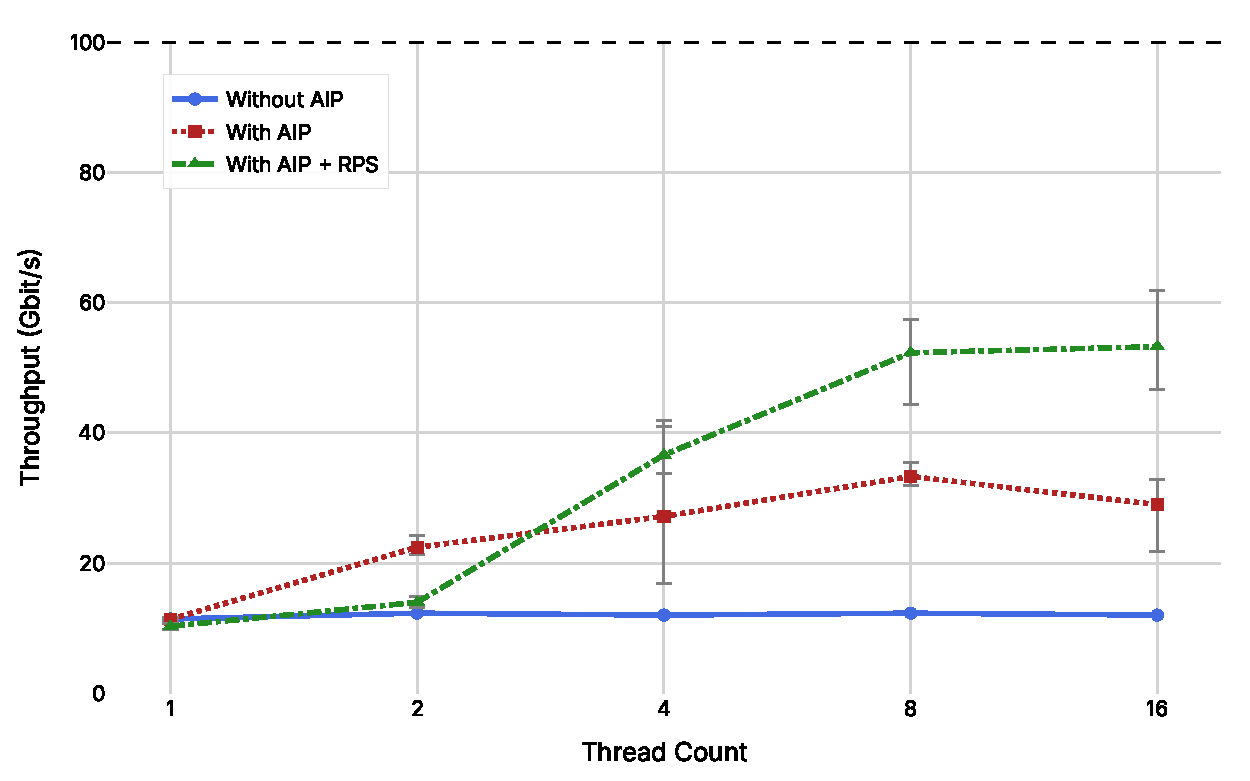
\includegraphics[width=1.0\linewidth]{assets/network/iperf/iperf_omnipath.pdf}
    \caption[Omni-Path TCP Throughput]{\acs{TCP} throughput over Omni-Path, measured using iperf2 with different parallelism settings. Despite the Accelerated \acs{IP} + \acs{RPS} method improving performance at high parallelism, the network link is underutilized.}
    \label{fig:opa-tcp-throughput}
\end{figure}

The lower performance at low thread counts with \ac{RPS} is consistent across runs. This is possibly due to the overhead of \ac{RPS} itself: the loss of cache locality and overhead of inter-processor interrupts caused by moving work to different cores may only be outweighed if the \ac{CPU} overhead of packet processing exceeds the capabilities of a single core.

As we suspect that Omni-Path performance depends highly on the performance of a single core, we performed additional testing of Omni-Path performance on consumer-grade hardware consisting of two systems, each with the hardware configuration shown in~\cref{tbl:validation-system}. These systems have the advantage over the server-grade system in that although it has less processing power overall, the per-core performance is higher; we should be able to determine if per-core performance is a bottleneck by running the benchmarks on this hardware.

\begin{table}[h]
\centering
\begin{tabular}{|ll|}
\hline
\textbf{Component} & \textbf{Specification} \\
\hline
CPU        & AMD Ryzen 9 5950X (16C/32T) \\
RAM        & 64 GB \\
Networking & 100 Gbit/s Omni-Path \\
\hline
% \multicolumn{2}{|l|}{\textbf{Memory Bandwidth Results}} \\
% \hline
% Theoretical    & 51.2 GB/s \\
% Measured       & 37.3 GB/s \\
% \hline
\end{tabular}
\caption{Validation System Hardware}
\label{tbl:validation-system}
\end{table}

Due to the limited number of cores, the number of \ac{SDMA} engines was reduced to 4, which necessitated reducing the parameter \texttt{num\_vls} to 4 as well. Accelerated \ac{IP} was enabled, and the number of user contexts was adjusted such that 6 \ac{IP} contexts were created, leaving 3 physical cores available for other tasks. The kernel parameters required to achieve this configuration are shown in~\cref{tbl:validation-system-kernel-opts}.

\begin{table}[h]
    \centering
    \begin{tabular}{|ll|}
        \hline
        \textbf{Parameter} & \textbf{Value} \\
        \hline
        \texttt{hfi1.num\_vls} & 4 \\
        \texttt{hfi1.num\_sdma} & 4 \\
        \texttt{hfi1.krcvqs} & 2 \\
        \texttt{hfi1.num\_user\_contexts} & 151 \\
        \texttt{hfi1.cap\_mask} & \texttt{0x4c09a09cbba} \\
        \hline
    \end{tabular}
    \caption[Kernel Parameters for Validation System]{Kernel parameters used for the validation system.}
    \label{tbl:validation-system-kernel-opts}
\end{table}

The interrupt layout of the validation system is shown in~\cref{fig:validation-system-irq}.

\begin{figure}[h]
    \centering
    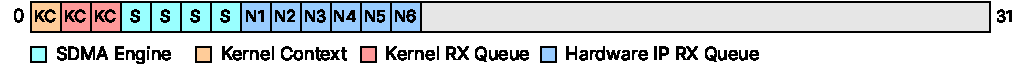
\includegraphics[width=\linewidth]{assets/network/rps/Interrupt-Layout-Ryzen.pdf}
    \caption[Validation System Interrupt Layout]{Interrupt layout of the validation system.}
    \label{fig:validation-system-irq}
\end{figure}

\Cref{fig:ryzen-opa-tcp-throughput} demonstrates the iperf throughput of the validation system with the adjusted kernel parameters and without \ac{RPS}, compared to the \ac{HPC} nodes with and without \ac{RPS}. In both cases, the validation system delivers much greater throughput than that of the \ac{HPC} nodes. However, the variance is still high: the 4-thread runs delivered between 65--93 Gbps of throughput.

\begin{figure}[H]
    \centering
    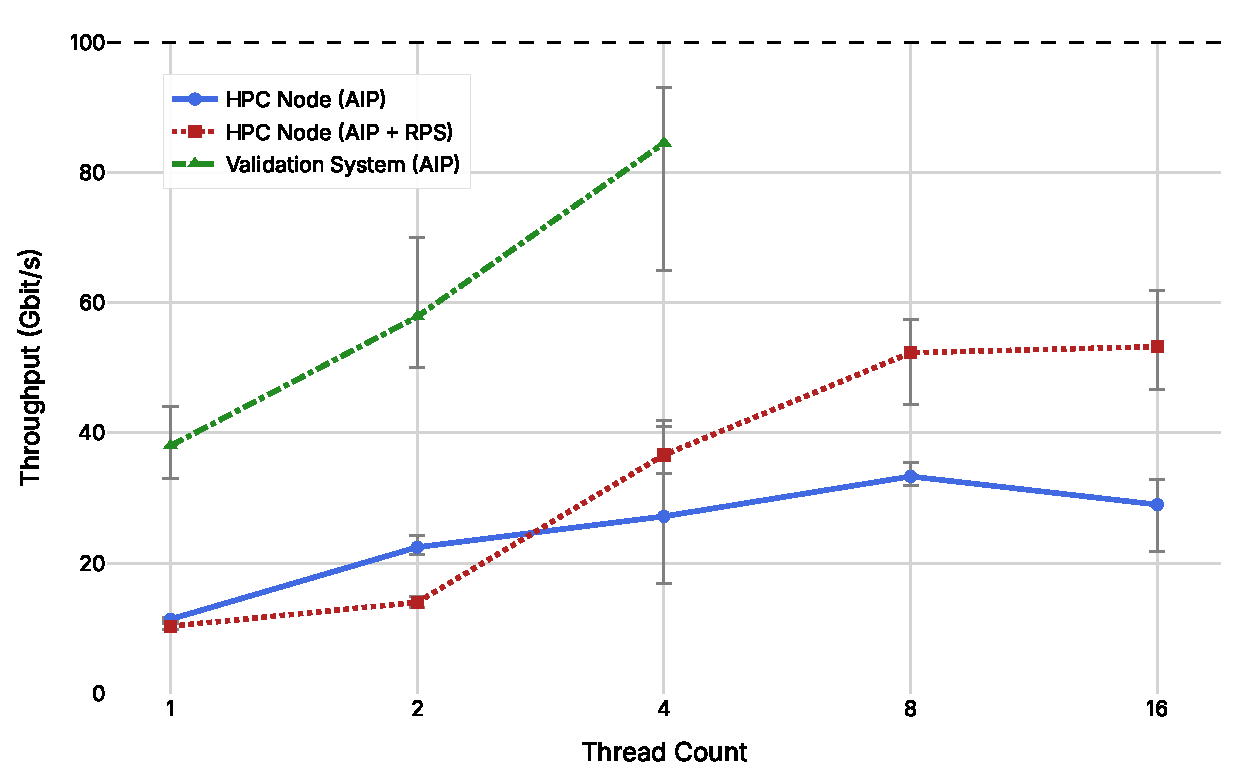
\includegraphics[width=\linewidth]{assets/network/iperf/iperf_comparison_rps_ryzen.pdf}
    \caption[Validation System TCP Performance]{\acs{TCP} throughput of the validation system. The validation systems' \ac{TCP} throughput is significantly higher than that of the \acs{HPC} nodes.}
    \label{fig:ryzen-opa-tcp-throughput}
\end{figure}

\subsubsection{InfiniBand}
\label{sec:results-network-bandwidth-ib}

\begin{figure}[H]
    \centering
    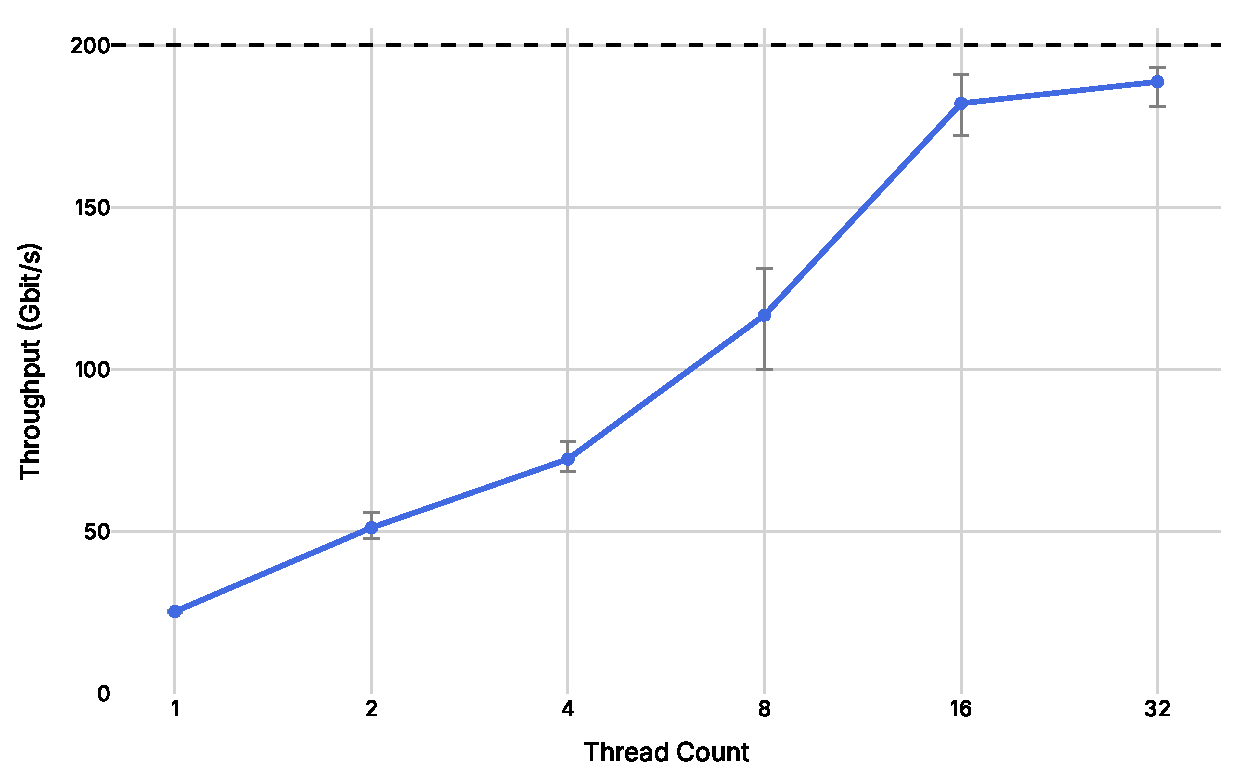
\includegraphics[width=1.0\linewidth]{assets/network/iperf/iperf_infiniband.pdf}
    \caption[InfiniBand TCP Throughput]{TCP throughput over InfiniBand, measured using iperf2 with different parallelism settings. The higher parallelism settings are capable of saturating the network link.}
    \label{fig:ib-tcp-throughput}
\end{figure}

The collected throughput results for InfiniBand are shown in~\cref{fig:ib-tcp-throughput}. A single thread achieved approximately 25 Gbit/s, whereas thread counts at or above 16 approached the theoretical network bandwidth limit of the network adapter. The peak observed throughput was 193 Gbit/s with 32 threads, representing 96.5\% of the 200 Gbit/s link speed.

During performance tests with lower thread counts, we observed iperf threads with 100\% \ac{CPU} utilization. This \ac{CPU} saturation suggests a bottleneck due to single-core processing performance, rather than a limitation of network capacity. As a result, we conclude that \ac{TCP} traffic is capable of saturating the physical network link given sufficient parallelism.

\subsection{Network Latency}

\begin{sloppypar}
For our standard network stack latency results, we used the Libfabric fi\_pingpong tool with the following options: \texttt{fi\_pingpong -e msg -I 1000} with \texttt{-p verbs} for \ac{RDMA} and \texttt{-p tcp} for \ac{TCP}, and either \texttt{-S} for message sizes of 64, 4096 (4\,KiB), or 134217728 (128\,MiB). The results are shown in~\cref{tbl:pingpong-latency} for the InfiniBand test system and~\cref{tbl:pingpong-latency-opa} for the Omni-Path test system. Note that 128\,MiB is provided as a network bandwidth test, rather than a latency test, in order to confirm \ac{RDMA} networking bandwidth.
\end{sloppypar}

\begin{table}[H]
\centering
\begin{tabular}{|lrrrr|}
\hline
\textbf{Transport} & \textbf{Size} & \textbf{Latency (\textmu{}s)} & \textbf{Bandwidth (MB/s)} & \textbf{Messages/sec} \\
\hline
\multirow{3}{*}{verbs} & 64   & 3.44  & 18.58 & 290,698.00 \\
                        & 4\,KiB   & 4.90  & 836.69 & 204,082.00 \\
                        & 128\,MiB & 6,863.50 & 19,555.30 & 145.00 \\
\multirow{3}{*}{tcp}   & 64   & 23.01  & 2.78 & 43,459.37 \\
                        & 4\,KiB   & 33.64  & 121.77 & 29,726.51 \\
                        & 128\,MiB & 60,724.00 & 2,210.30 & 16.47 \\
\hline
\end{tabular}
\caption[InfiniBand Latency Results]{Network latency results for the InfiniBand test system.}
\label{tbl:pingpong-latency}
\end{table}

\begin{table}[H]
\centering
\begin{tabular}{|lrrrr|}
\hline
\textbf{Transport} & \textbf{Size} & \textbf{Latency (\textmu{}s)} & \textbf{Bandwidth (MB/s)} & \textbf{Messages/sec} \\
\hline
\multirow{3}{*}{verbs} & 64   & 7.61  & 8.41 & 131,406.04 \\
                        & 4\,KiB   & 9.95  & 411.45 & 100,502.51 \\
                        & 128\,MiB & 27,558.80 & 4,644.75 & 36.29 \\
\multirow{3}{*}{tcp}   & 64   & 18.53  & 3.45 & 53,966.54 \\
                        & 4\,KiB   & 29.57  & 138.51 & 33,818.06 \\
                        & 128\,MiB & 130,347.60 & 1,029.69 & 7.68 \\
\hline
\end{tabular}
\caption[Omni-Path Latency Results]{Network latency results for the Omni-Path test system.}
\label{tbl:pingpong-latency-opa}
\end{table}

Overall, the InfiniBand system delivers better performance than the Omni-Path system, with lower latency and higher bandwidth, with the exception of small-message \ac{TCP} performance, where Omni-Path outperforms InfiniBand. For both transports, the \ac{RDMA} performance is higher than \ac{TCP} performance. We expect that, based on these results, latency-sensitive Ceph workloads will benefit most from \ac{RDMA} networking. Additionally, because these tests were performed with a single thread, we also expect that single-task operations will be significantly faster on the \ac{RDMA} backend than \ac{TCP}. These latency results primarily serve as our upper bound for per-client \ac{IOPS} performance results.

\subsection{Memory Bandwidth}

Memory bandwidth limits were measured using the Intel Memory Latency Checker on the Intel Omni-Path system and pmbw on the AMD InfiniBand system due to its inability to run correctly on the latter. Theoretical memory bandwidth results are collected from the data sheets for the respective processors\footnote{InfiniBand/AMD System: \url{https://www.amd.com/en/products/processors/server/epyc/7003-series/amd-epyc-7513.html}; Omni-Path/Intel System: \url{https://www.intel.de/content/www/de/de/products/sku/231735/intel-xeon-platinum-8468-processor-105m-cache-2-10-ghz/specifications.html}. Accessed 23.02.2026.}. Theoretical memory bandwidth was calculated using \ac{DRAM} Speed in MT/s $\times$ 8 $\times$ channel count if memory bandwidth was not explicitly specified in the product specifications.

\begin{table}[H]
\centering
\begin{tabular}{|llll|}
\hline
\textbf{Test System Type} & \textbf{Theoretical} & \textbf{Peak Read (GiB/s)} & \textbf{Peak Write (GiB/s)} \\
\hline
InfiniBand & 409.60* & 140.91 & 82.32 \\
Omni-Path & 614.40* & 494.04 & 350.92 \\
Omni-Path (pmbw) & 614.40* & 194.14 & 152.97 \\
\hline
\end{tabular}

\smallskip
\small{
    * Total system memory bandwidth across both \acs{CPU}s.
}

\caption[Peak Memory Bandwidth Results]{Peak memory bandwidth results for the InfiniBand and Omni-Path test systems.}
\label{tbl:peak-memory-bandwidth}
\end{table}

Note that the bandwidth measured using pmbw is likely an underestimate of the true memory bandwidth; the tool is not as optimized as the Intel Memory Latency Checker, and running pmbw on the Omni-Path system produced similarly low results. However, the results are sufficient to determine that the network, not memory bandwidth, is the primary  bottleneck for the Ceph benchmarks.



%%%%%%%%%%%%%%%%%%%%%%%%%%%%%%%%%%

\subsection{Disk Performance}

As our in-memory cluster is not equipped with physical disks, we do not consider disk performance when considering bottlenecks for these results. However, we have measured the disk performance scaling in our controlled virtual machine environment, in order to determine how disk performance scales depending on the number of objects, replication policy, and placement group count. We will compare our hypothesized results with our observed scaling results.

Our hypothesis based on Ceph's operational characteristics and our cluster configuration of 8 \acp{OSD} and 50 MiB/s rate limiting per \ac{OSD} is shown in~\cref{tbl:disk-performance-hypothesis}.

\begin{table}[htbp]
\centering
\begin{tabular}{|l|l|l|}
\hline
\textbf{Pool Type} & \textbf{Read} & \textbf{Write} \\
\hline
Replicated (size $x$) & min(\acs{PG}, 8) $\times$ 50 & min(\acs{PG} $\times$ 50, $\sfrac{400}{x}$) \\
\hline
\acs{EC} ($k + m$) & min($k \times$ \acs{PG}, 8) $\times$ 50 & min(($k + m$) $\times$ \acs{PG}, 8) $\times$ 50 $\times$ $\sfrac{k}{(k+m)}$ \\
\hline
\end{tabular}
\caption[Disk Performance Hypothesis]{Disk performance hypothesis for the Ceph cluster.}
\label{tbl:disk-performance-hypothesis}
\end{table}

It should be noted that the implementation of our throttling method\footnote{\url{https://github.com/qemu/qemu/blob/a17976b04f2117e1bab64358f873b36fe4561520/docs/throttle.txt\#L218}. Accessed 26.02.2026.} may result in higher burst performance. This is likely to favor \ac{EC} pools with higher disk counts, as each \ac{OSD} must read less data, making burst performance a larger share of the total performance. We have attempted to mitigate this by using \ac{I/O} operations which result in benchmark runtimes of several seconds. Therefore, this implicit benefit should be taken into consideration when considering the results. Additionally, the pseudorandom distribution of objects across \acp{PG} may result in the uneven distribution of objects across \acp{OSD}, leading to lower performance as disks are underutilized. 

\subsubsection{128-\acs{PG} Read Performance Scaling}

\begin{figure}[H]
    \centering
    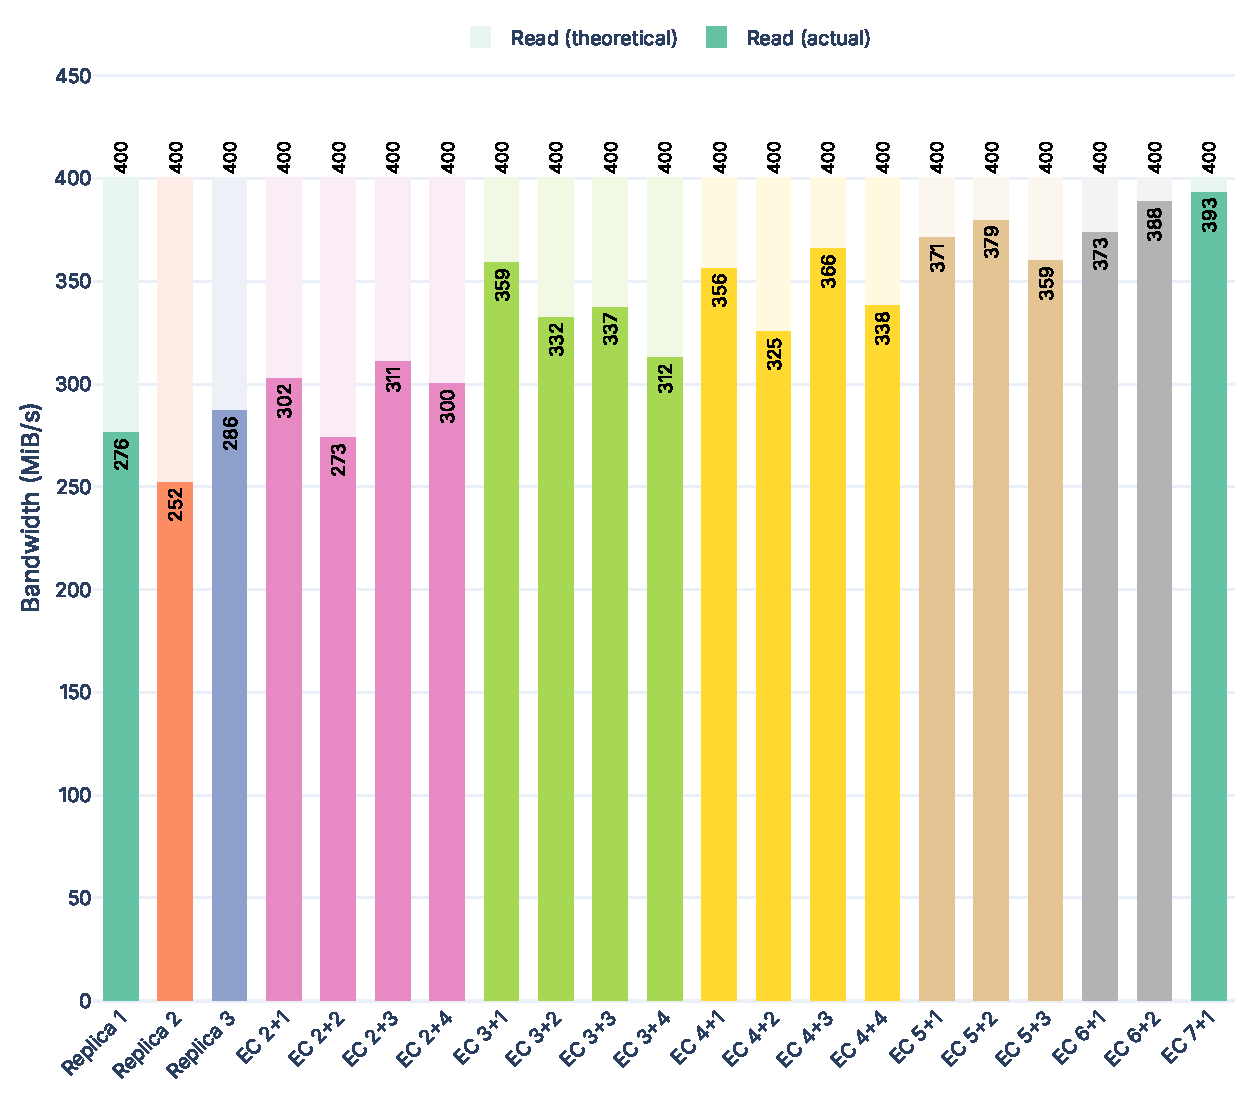
\includegraphics[width=\textwidth]{assets/perf_results/lab_128pg_read.pdf}
    \caption[128-\acs{PG} Read Performance Scaling]{Read performance scaling for 128 \acs{PG} pools with various replication and erasure coding profiles.}
    \label{fig:128pg-read-scaling}
\end{figure}

\Cref{fig:128pg-read-scaling} shows the read performance with 128 \acp{PG}. Since 128 \acp{PG} should be sufficient to distribute objects across all \acp{OSD}, the read performance should be limited by the cluster's combined throughput of 400\,MiB/s. Replication factor has no significant impact on read throughput; however, we only observed up to $\approx$ 286\,MiB/s, or 71.5\%, of the cluster's performance limit. Pools with \ac{EC} show strong performance characteristics, better than those of replicated pools, with the highest 7+1 \ac{EC} profile reaching close to the theoretical maximum.

\pagebreak
\subsubsection{128-\acs{PG} Write Performance Scaling}

\begin{figure}[H]
    \centering
    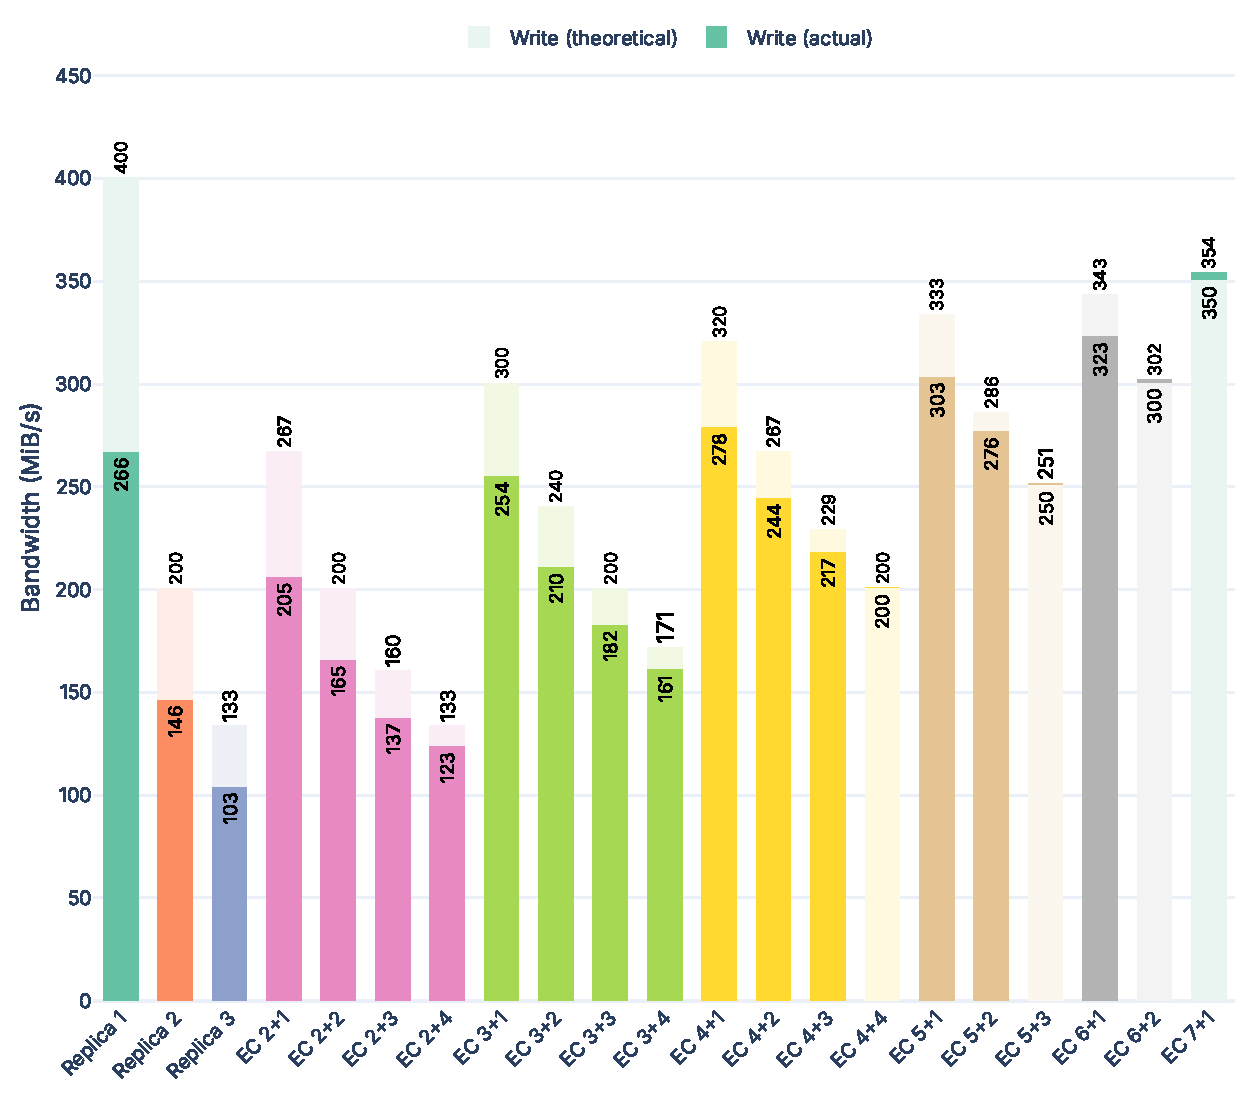
\includegraphics[width=\textwidth]{assets/perf_results/lab_128pg_write.pdf}
    \caption[128-\acs{PG} Write Performance Scaling]{Write performance scaling for 128 \acs{PG} pools with various replication and erasure coding profiles.}
    \label{fig:128pg-write-scaling}
\end{figure}

\Cref{fig:128pg-write-scaling} shows the write performance with 128 \acp{PG}. For replicated pools, the total throughput is divided by the replication factor, while for \ac{EC} pools, the write throughput is limited by the number of total coding chunks. Overall, we observed that the replicated pools achieved about 70--80\% of the block device limit, while \ac{EC} pools generally outperformed the replicated pools both in terms of efficiency and overall throughput at the same level of failure tolerance.

\pagebreak
\subsubsection{Single-\acs{PG} Read Performance Scaling}

\begin{figure}[H]
    \centering
    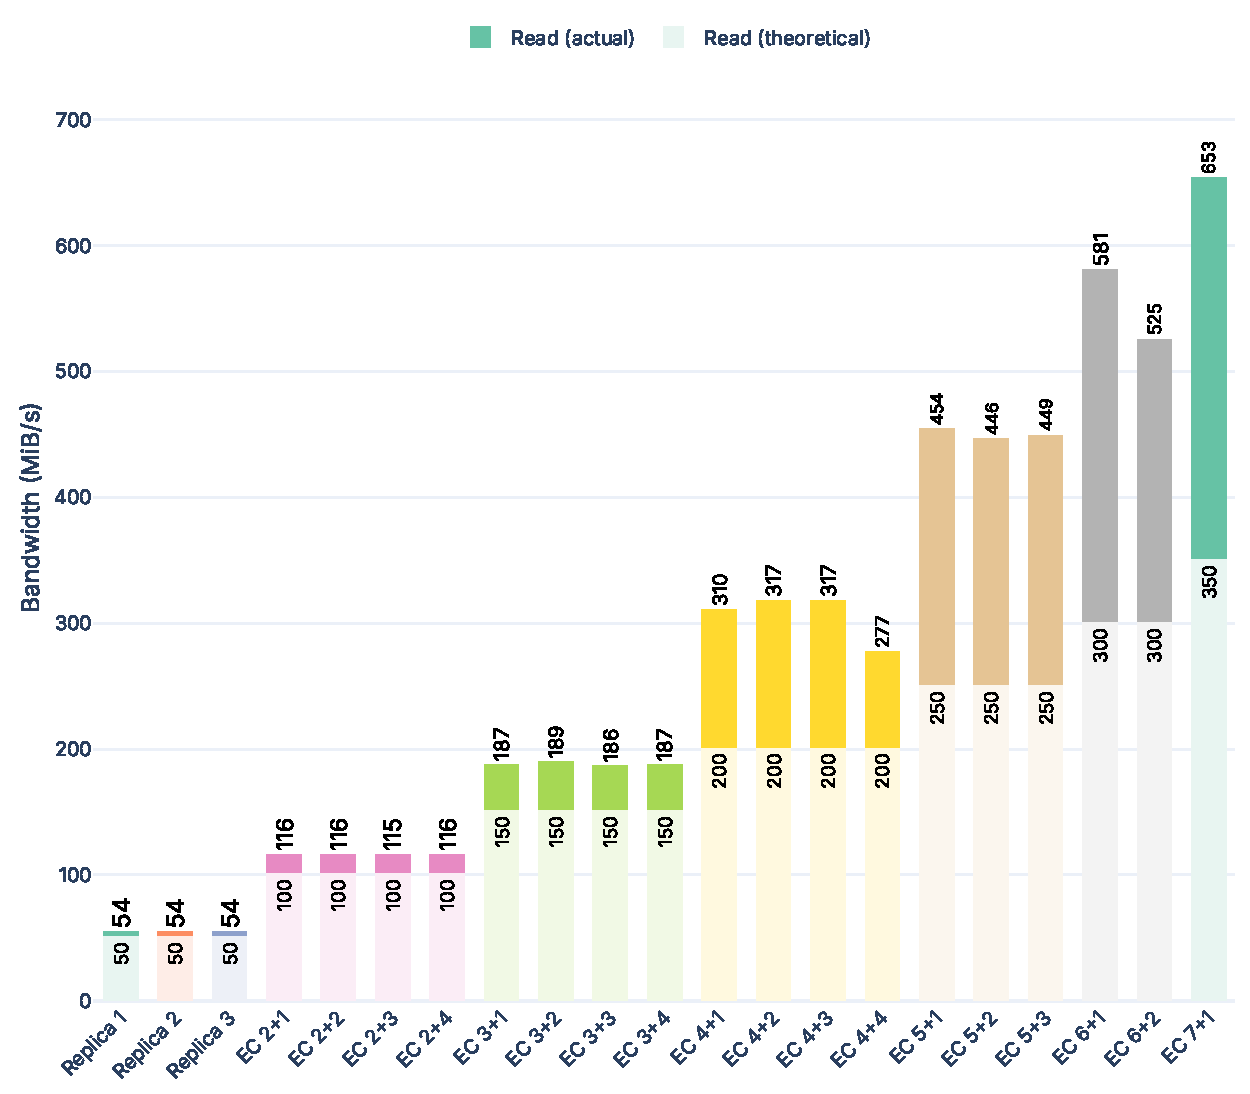
\includegraphics[width=\textwidth]{assets/perf_results/lab_1pg_read.pdf}
    \caption[Single-\acs{PG} Read Performance Scaling]{Read performance scaling for a single 
    \acs{PG} pool with various replication and erasure coding profiles.}
    \label{fig:1pg-read-scaling}
\end{figure}

\Cref{fig:1pg-read-scaling} shows read performance with a single \acs{PG}. Single-\acs{PG} pools, or single-object writes to multi-\acs{PG} pools, are a weak spot for replicated pools, as they are limited by the per-\acs{OSD} rate limit.

\subsubsection{Single-\acs{PG} Write Performance Scaling}

\begin{figure}[H]
    \centering
    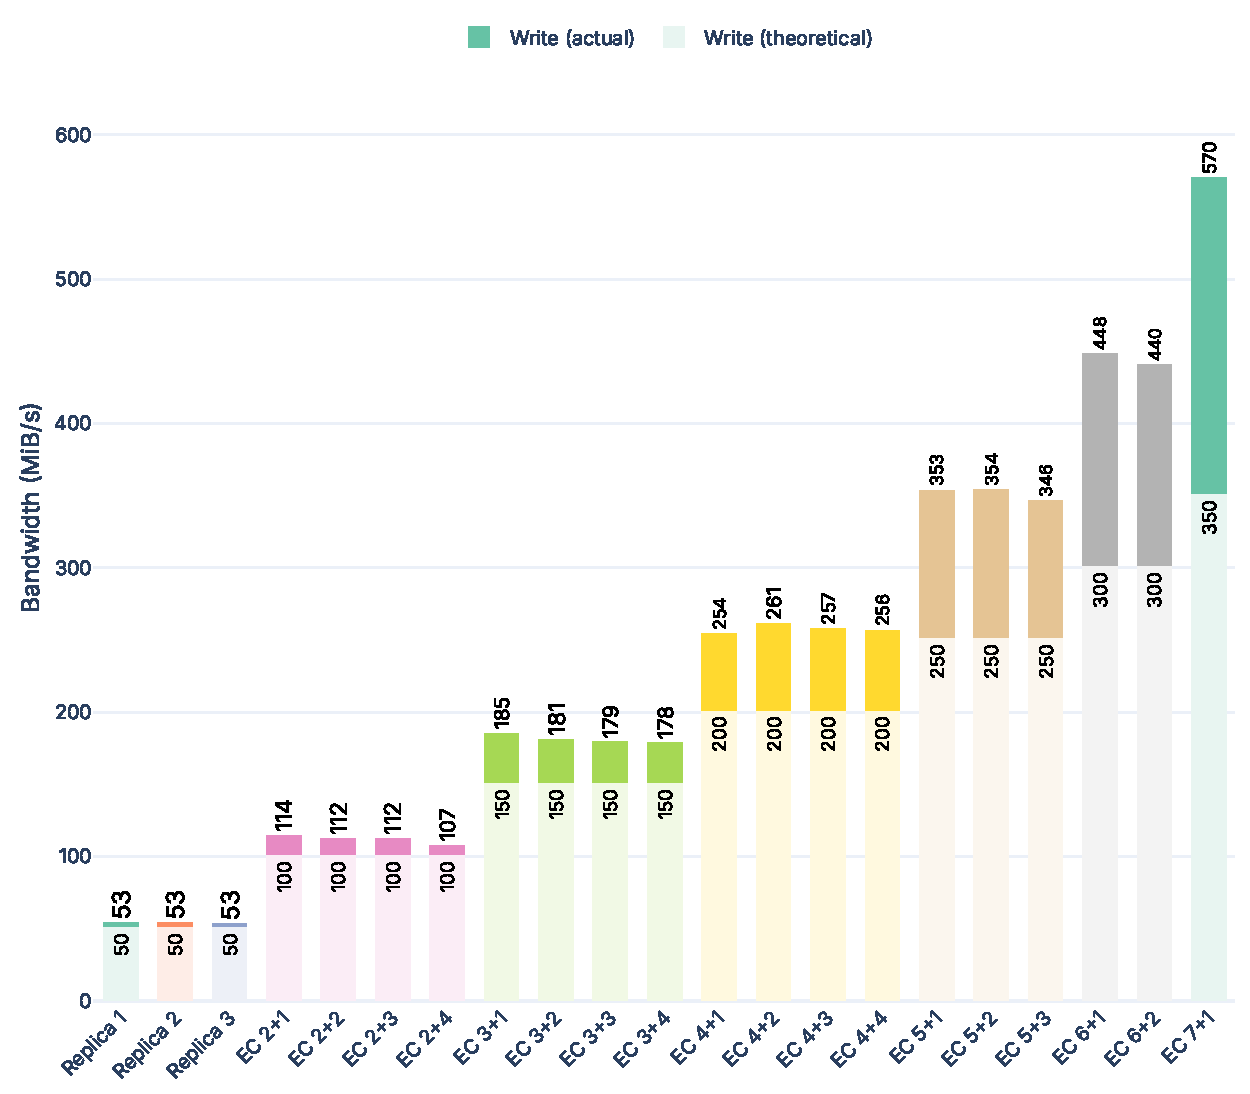
\includegraphics[width=\textwidth]{assets/perf_results/lab_1pg_write.pdf}
    \caption[Single-\acs{PG} Write Performance Scaling]{Write performance scaling for a single 
    \acs{PG} pool with various replication and erasure coding profiles.}
    \label{fig:1pg-write-scaling}
\end{figure}

\Cref{fig:1pg-write-scaling} shows write performance with a single \acs{PG}. Performance results are similar to the read performance, with replicated pools again showing flat throughput regardless of the replication factor and all pools showing higher actual performance results than the theoretical limit. As noted earlier, this is likely attributable to the burst behaviour of the throttling implementation.